% !TEX TS-program = pdflatex

% !TEX encoding = UTF-8 Unicode



% This is a simple template for a LaTeX document using the "article" class.

% See "book", "report", "letter" for other types of document.



\documentclass[8pt]{article} % use larger type; default would be 10pt



\usepackage[utf8]{inputenc} % set input encoding (not needed with XeLaTeX)

\usepackage{bchart}

\usepackage{longtable}

\usepackage{pgfgantt}

\usepackage{calendar} % Use the calendar.sty style

\usepackage{calc}

\usepackage{ifthen}

\usepackage{tkz-base}





%%% Examples of Article customizations

% These packages are optional, depending whether you want the features they provide.

% See the LaTeX Companion or other references for full information.



\usepackage{textcomp}

%\usepackage{hyperref}



%%% PAGE DIMENSIONS

\usepackage{geometry} % to change the page dimensions

\geometry{a4paper} % or letterpaper (US) or a5paper or....

% \geometry{margin=2in} % for example, change the margins to 2 inches all round

% \geometry{landscape} % set up the page for landscape

%   read geometry.pdf for detailed page layout information



\usepackage{graphicx} % support the \includegraphics command and options



% \usepackage[parfill]{parskip} % Activate to begin paragraphs with an empty line rather than an indent



%%% PACKAGES

\usepackage{booktabs} % for much better looking tables

\usepackage{array} % for better arrays (eg matrices) in maths

\usepackage{paralist} % very flexible & customisable lists (eg. enumerate/itemize, etc.)

\usepackage{verbatim} % adds environment for commenting out blocks of text & for better verbatim

\usepackage{subfig} % make it possible to include more than one captioned figure/table in a single float

% These packages are all incorporated in the memoir class to one degree or another...



%%% HEADERS & FOOTERS

\usepackage{fancyhdr} % This should be set AFTER setting up the page geometry

\pagestyle{fancy} % options: empty , plain , fancy

\renewcommand{\headrulewidth}{0pt} % customise the layout...

\lhead{}\chead{}\rhead{}

\lfoot{}\cfoot{\thepage}\rfoot{}



%%% SECTION TITLE APPEARANCE

\usepackage{sectsty}

\allsectionsfont{\sffamily\mdseries\upshape} % (See the fntguide.pdf for font help)

% (This matches ConTeXt defaults)



%%% ToC (table of contents) APPEARANCE

\usepackage[nottoc,notlof,notlot]{tocbibind} % Put the bibliography in the ToC

\usepackage[titles,subfigure]{tocloft} % Alter the style of the Table of Contents

\renewcommand{\cftsecfont}{\rmfamily\mdseries\upshape}

\renewcommand{\cftsecpagefont}{\rmfamily\mdseries\upshape} % No bold!



%%% END Article customizations



%%% The "real" document content comes below...



\title{Personal}

\author{\copyright Frederic Kerdraon}

%\date{} % Activate to display a given date or no date (if empty),

         % otherwise the current date is printed 



\begin{document}

\maketitle

\tableofcontents



\section{Introduction}



This document summurizes all the important informations necessary to facilitate things and remove a lot of stress. It's been put together thanks to \LaTeX. This is designed to help make optimal decisions for a not so short lifetime.



{\footnotesize

Ce n'est pas parceque les choses sont difficiles que nous n'osons pas, c'est parceque nous n'osons pas qu'elles sont difficiles.

}

%\makebox[2\width]{hello}

% !TEX TS-program = pdflatex
% !TEX encoding = UTF-8 Unicode

% This is a simple template for a LaTeX document using the "article" class.
% See "book", "report", "letter" for other types of document.

\documentclass[8pt]{article} % use larger type; default would be 10pt

\usepackage[utf8]{inputenc} % set input encoding (not needed with XeLaTeX)
\usepackage{bchart}
\usepackage{longtable}
\usepackage{pgfgantt}
\usepackage{calendar} % Use the calendar.sty style
\usepackage{calc}
\usepackage{ifthen}
\usepackage{tkz-base}
\usepackage{pdfpages}
\usepackage{hyperref}
%%% Examples of Article customizations
% These packages are optional, depending whether you want the features they provide.
% See the LaTeX Companion or other references for full information.

\usepackage{textcomp}
%\usepackage{hyperref}

%%% PAGE DIMENSIONS
\usepackage{geometry} % to change the page dimensions
\geometry{a4paper} % or letterpaper (US) or a5paper or....
% \geometry{margin=2in} % for example, change the margins to 2 inches all round
% \geometry{landscape} % set up the page for landscape
%   read geometry.pdf for detailed page layout information

\usepackage{graphicx} % support the \includegraphics command and options

% \usepackage[parfill]{parskip} % Activate to begin paragraphs with an empty line rather than an indent

%%% PACKAGES
\usepackage{booktabs} % for much better looking tables
\usepackage{array} % for better arrays (eg matrices) in maths
\usepackage{paralist} % very flexible & customisable lists (eg. enumerate/itemize, etc.)
\usepackage{verbatim} % adds environment for commenting out blocks of text & for better verbatim
\usepackage{subfig} % make it possible to include more than one captioned figure/table in a single float
% These packages are all incorporated in the memoir class to one degree or another...

%%% HEADERS & FOOTERS
\usepackage{fancyhdr} % This should be set AFTER setting up the page geometry
\pagestyle{fancy} % options: empty , plain , fancy
\renewcommand{\headrulewidth}{0pt} % customise the layout...
\lhead{}\chead{}\rhead{}
\lfoot{}\cfoot{\thepage}\rfoot{}

%%% SECTION TITLE APPEARANCE
\usepackage{sectsty}
\allsectionsfont{\sffamily\mdseries\upshape} % (See the fntguide.pdf for font help)
% (This matches ConTeXt defaults)

%%% ToC (table of contents) APPEARANCE
\usepackage[nottoc,notlof,notlot]{tocbibind} % Put the bibliography in the ToC
\usepackage[titles,subfigure]{tocloft} % Alter the style of the Table of Contents
\renewcommand{\cftsecfont}{\rmfamily\mdseries\upshape}
\renewcommand{\cftsecpagefont}{\rmfamily\mdseries\upshape} % No bold!

%%% END Article customizations

%%% The "real" document content comes below...

\title{Management documentation}
\author{\copyright Frederic Kerdraon}
%\date{} % Activate to display a given date or no date (if empty),
         % otherwise the current date is printed 

\begin{document}
\maketitle
\tableofcontents

\newcounter{a}
\newcounter{b}
%----------------------------------------------------------
\newcommand{\slice}[4]{
  \pgfmathparse{0.5*#1+0.5*#2}
  \let\midangle\pgfmathresult

   slice
  \draw[thick,fill=black!10] (0,0) -- (#1:1) arc (#1:#2:1) -- cycle;

   outer label
  \node[label=\midangle:#4] at (\midangle:1) {};

   inner label
  \pgfmathparse{min((#2-#1-10)/110*(-0.3),0)}
  \let\temp\pgfmathresult
  \pgfmathparse{max(\temp,-0.5) + 0.8}
  \let\innerpos\pgfmathresult
  \node at (\midangle:\innerpos) {#3};
}

\section{Management summary}



\begin{longtable}{|c|c|c|c|c|}
\hline
\multicolumn{5}{|c|}{Contacts} \\
\hline
ID & Name & Rating & Town & Telephone\\
\hline
101 & Wing & 1000 & HongKong & 85296001395\\
\hline
108 & Zazzy & 900 & Brest & 33611037735\\
\hline
27 & Flozio & 850 & Brest & 33680938975\\
\hline
24 & Fanch & 800 & Brest & 33685769214\\
\hline
68 & Mummy & 800 & Brest & 33674340108\\
\hline
89 & Sonia & 600 & Rennes & 33612425946\\
\hline
83 & Rico & 550 & Brest & 33611037992\\
\hline
60 & Maeva & 500 & Brest & 33662575512\\
\hline
42 & Jessie & 500 & Brest & 33681775660\\
\hline
41 & Jessica & 500 & Brest & 699114929\\
\hline
23 & Etienne & 400 & Brest & 619144832\\
\hline
2 & Armelle & 400 & Brest & 33677134026\\
\hline
96 & Tiprig & 250 & Paris & 33663626188\\
\hline
22 & Elise & 250 & ???? & 33614921085\\
\hline
 ... & ... & ... & ... & ... \\
\hline
Total & 8300 &  & & \\
\hline
\end{longtable}

%\subsection{Weekly calendar}



%{\footnote

%Pour tous les items il faudrait un mail de rappel comme pour les livrables, meetings et vacances

%}



\begin{calendar}{\hsize}



%----------------------------------------------------------------------------------------

%	FIRST DAY

%----------------------------------------------------------------------------------------



\day{}{

09:15-10:15 \daysep \textbf{Messe}\\[3pt]

\textbf{10am-12am} \daysep Marche\\[3pt]

\textbf{12am-2pm} \daysep Dejeuner maison\\[3pt]

\textbf{7pm-9pm} \daysep Canal football club\\[3pt]

\textbf{9pm-11pm} \daysep Guitar\\[3pt]

\textbf{12am-2pm} \daysep Muscu\\[3pt]

}

% By default all daily events are centered in the box, in order to bring them up use \vspace{2cm} after the event text; you may need to change the 2cm



%----------------------------------------------------------------------------------------

%	SECOND DAY

%----------------------------------------------------------------------------------------



\day{}{

\textbf{9am-10am} \daysep Preparation cours de math \\[3pt]

\textbf{10am-12am} \daysep Preparation presentation finance \\[3pt]

\textbf{1pm-2pm} \daysep Manage my weekly \\[3pt]

\textbf{2pm-4pm} \daysep Administration \\[3pt]

\textbf{4pm-5pm} \daysep Lessive \\[3pt]

\textbf{7pm-10pm} \daysep Cinema \\[3pt]

%\textbf{9am-10am} \daysep BIOSCI101 - BLT100 \\[3pt]

%\textbf{10am-11am} \daysep BIOSCI 104 - LLT \\[3pt]

%\textbf{11am-12pm} \daysep No Lecture \\[3pt]

%\textbf{12pm-1pm} \daysep No Lecture \\[3pt]

%\textbf{12pm-1pm} \daysep BIOSCI105 - BLT204 \\[3pt]

%\textbf{1pm-2pm} \daysep No Lecture \\[3pt]

%\textbf{3pm-4pm} \daysep BIOSCI101 Laboratory \\[3pt]

%\textbf{4pm-5pm} \daysep BIOSCI101 Laboratory

} 



%----------------------------------------------------------------------------------------

%	THIRD DAY

%----------------------------------------------------------------------------------------



\day{}{ % Tuesday

\textbf{9am-10am} \daysep Preparation cours de math \\[3pt]

\textbf{10am-12am} \daysep Preparation presentation finance \\[3pt]

\textbf{10am-12am} \daysep Bibliotheque \\[3pt]

\textbf{10am-12am} \daysep Validation of finances\\[3pt]

\textbf{7pm-9pm} \daysep Krav maga \\[3pt]

%\textbf{3pm-4pm} \daysep No Lecture \\[3pt]

%\textbf{4pm-5pm} \daysep No Lecture

} 



%----------------------------------------------------------------------------------------

%	FOURTH DAY

%----------------------------------------------------------------------------------------



\day{}{ % Wednesday

\textbf{9am-10am} \daysep Preparation cours de math \\[3pt]

\textbf{10am-12am} \daysep Preparation presentation finance \\[3pt]

%\textbf{9am-10am} \daysep No Lecture \\[3pt]

%\textbf{10am-11am} \daysep BIOSCI 104 - LLT \\[3pt]

%\textbf{11am-12pm} \daysep No Lecture \\[3pt]

%\textbf{12pm-1pm} \daysep BIOSCI105 - BLT204 \\[3pt]

%\textbf{1pm-2pm} \daysep No Lecture \\[3pt]

%\textbf{2pm-3pm} \daysep GEO101 - HSB1 \\[3pt]

\textbf{7pm-10pm} \daysep Football \\[3pt]

%\textbf{3pm-4pm} \daysep No Lecture \\[3pt]

%\textbf{4pm-5pm} \daysep No Lecture

} 



%----------------------------------------------------------------------------------------

%	FIFTH DAY

%----------------------------------------------------------------------------------------



\day{}{ % Thursday

\textbf{9am-10am} \daysep Preparation cours de math \\[3pt]

\textbf{10am-12am} \daysep Preparation presentation finance \\[3pt]

\textbf{7pm-9pm} \daysep Krav maga \\[3pt]

%\textbf{9am-10am} \daysep No Lecture \\[3pt]

%\textbf{10am-11am} \daysep BIOSCI 104 - LLT \\[3pt]

%\textbf{11am-12pm} \daysep No Lecture \\[3pt]

%\textbf{12pm-1pm} \daysep No Lecture \\[3pt]

%\textbf{1pm-2pm} \daysep No Lecture \\[3pt]

%\textbf{2pm-3pm} \daysep GEO101 - HSB1 \\[3pt]

%\textbf{3pm-4pm} \daysep No Lecture \\[3pt]

%\textbf{4pm-5pm} \daysep No Lecture

} 



%----------------------------------------------------------------------------------------

%	SIXTH DAY

%----------------------------------------------------------------------------------------



\day{}{ % Friday

\textbf{9am-10am} \daysep Preparation cours de math \\[3pt]

\textbf{10am-12am} \daysep Preparation presentation finance \\[3pt]

\textbf{12am-2pm} \daysep Badminton \\[3pt]

\textbf{9pm-11pm} \daysep Drinks \\[3pt]

%\textbf{10am-11am} \daysep BIOSCI 104 - LLT \\[3pt]

%\textbf{11am-12pm} \daysep No Lecture \\[3pt]

%\textbf{12pm-1pm} \daysep BIOSCI105 - BLT204 \\[3pt]

%\textbf{1pm-2pm} \daysep No Lecture \\[3pt]

%\textbf{2pm-3pm} \daysep No Lecture \\[3pt]

%\textbf{3pm-4pm} \daysep GEO101 Tutorial \\ Room A \\[3pt]

%\textbf{4pm-5pm} \daysep No Lecture

} 



%----------------------------------------------------------------------------------------

%	SEVENTH DAY

%----------------------------------------------------------------------------------------



\day{}{ % Saturday

\textbf{9am-10am} \daysep Preparation cours de math \\[3pt]

\textbf{10am-12am} \daysep Courses \\[3pt]

\textbf{2pm-4pm} \daysep Menage \\[3pt]

\textbf{4pm-9pm} \daysep Get back energy \\[3pt]

\textbf{9pm-11pm} \daysep Go dancing \\[3pt]

\textbf{9pm-11pm} \daysep Go sailing \\[3pt]

}

%----------------------------------------------------------------------------------------

 

\finishCalendar

\end{calendar}



\input{Events}
%\input{Map}
%\begin{longtable}{|c|c|c|c|c|c|c|}
\hline
\multicolumn{7}{|c|}{Tasks} \\
\hline
ID & Project & Task & Weight & Complexity & TheoEnd & EndDate\\
\hline
9 & "Pro" & "Donner mon numero de tel & 70 & 0 & 'toto' & 'toto'\\
\hline
8 & "Admin" & "Faire le virement HSBC" & 80 & 0 & 'toto' & 'toto'\\
\hline
6 & "Bateau" & "Carenner le bateau" & 90 & 0 & 'toto' & 'toto'\\
\hline
7 & "Day to day" & "Creer checklist depart B & 90 & 0 & 'toto' & 'toto'\\
\hline
3 & "Admin" & "Payer les impots" & 100 & 1 & 'toto' & 'toto'\\
\hline
4 & "Day to day" & "Se faire couper les chev & 100 & 1 & 'toto' & 'toto'\\
\hline
5 & "Life" & "Have fucking sex everyda & 100 & 1 & 'toto' & 'toto'\\
\hline
69 & "Communication" & "Etablir weeklies" & 300 & 0 & 'toto' & 'toto'\\
\hline
\end{longtable}

%\begin{longtable}{|c|c|c|}
\hline
\multicolumn{3}{|c|}{Mandatory Checks} \\
\hline
ID & Name & Checklist\\
\hline
51 & tentes & Week-end\\
\hline
52 & 2 underwares & Week-end\\
\hline
53 & 100 euro & Week-end\\
\hline
54 & some music & Week-end\\
\hline
55 & grosses chaussettes & Week-end\\
\hline
56 & marteau & Week-end\\
\hline
67 & Thermos & Week-end\\
\hline
68 & Carte & Week-end\\
\hline
69 & Tickets Reservations & Week-end\\
\hline
70 & Swiss knife & Week-end\\
\hline
71 & Guitar & Week-end\\
\hline
72 & Present hosts & Week-end\\
\hline
73 & Frontale & Week-end\\
\hline
74 & Montre g Shock & Week-end\\
\hline
75 & Petite serviette & Week-end\\
\hline
76 & Short de bain & Week-end\\
\hline
77 & Couteau Suisse & Week-end\\
\hline
91 & Couette & Week-end\\
\hline
92 & Oreiller & Week-end\\
\hline
93 & Thermos & Week-end\\
\hline
94 & Marteau & Week-end\\
\hline
95 & Sac poubelle & Week-end\\
\hline
96 & Affaires de sport & Week-end\\
\hline
97 & Couette & Week-end\\
\hline
98 & Couverts & Week-end\\
\hline
99 & Table pliante & Week-end\\
\hline
100 & Chaise pliante & Week-end\\
\hline
101 & Sac linge sale & Week-end\\
\hline
102 & Short & Week-end\\
\hline
103 & Glaciere elec & Week-end\\
\hline
104 & Boite dejeuner & Week-end\\
\hline
\end{longtable}

%\begin{longtable}{|c|c|c|c|c|c|}
\hline
\multicolumn{6}{|c|}{Skills} \\
\hline
ID & Contact & Name & Rating & Experience & Reference\\
\hline
23 & Fred & Football & 1000 & 0 & Louis\\
\hline
1 & Fred & Project-management & 850 & 0 & Mark\\
\hline
2 & Fred & Finance & 700 & 0 & Pete\\
\hline
3 & Fred & Risk-management & 550 & 0 & Pete\\
\hline
4 & Fred & Organisation & 400 & 0 & Phil\\
\hline
7 & Fred & Career-development & 250 & 0 & Toto\\
\hline
9 & Fred & Information-technology & 100 & 0 & Toto\\
\hline
13 & Fred & Sports & 90 & 0 & Toto\\
\hline
 ... & ... & ... & ... & ... & ... \\
\hline
 & & Total & 4502 &  & \\
\hline
\end{longtable}

%\begin{longtable}{|c|c|c|c|c|c|}
\hline
\multicolumn{6}{|c|}{Tasks} \\
\hline
Project & Task & Return & Cost & R/C & NumDays \\
\hline
Boat & Sell Plijadur & 15000 & 1 & 15000 & 10\\
\hline
IT & Qt - add global update for tasks from Qt & 1000 & 1 & 1000 & 10\\
\hline
Climate camp & visiter les terrains et poser des jalons & 750 & 1 & 750 & 10\\
\hline
Friends & Diner Armelle & 3200 & 5 & 640 & 10\\
\hline
Friends & Diner Christophe & 1200 & 2 & 600 & 10\\
\hline
Work & Meet guys fromTyfab & 500 & 1 & 500 & 10\\
\hline
Work & Meet guys fromTyfab & 500 & 1 & 500 & 10\\
\hline
Friends & D�jeuner Karel & 4000 & 10 & 400 & 10\\
\hline
Friends & Diner Zaz & 3800 & 10 & 380 & 10\\
\hline
Friends & Diner Jab & 400 & 2 & 200 & 10\\
\hline
Boat & Sale genoa36 & 150 & 1 & 150 & 10\\
\hline
Boat & Motor servicing & 100 & 1 & 100 & 10\\
\hline
Boat & Careen the Boat & 90 & 1 & 90 & 10\\
\hline
Finance & HSBC transfer & 80 & 1 & 80 & 10\\
\hline
Boat & Genoa - crowd funding? & 50 & 1 & 50 & 10\\
\hline
Plijadur & Plastify maps & 40 & 1 & 40 & 10\\
\hline
Plijadur & Plastify maps & 40 & 1 & 40 & 10\\
\hline
Boat & Buy masks & 40 & 1 & 40 & 10\\
\hline
Boat & Write log book - for history & 35 & 1 & 35 & 10\\
\hline
Plijadur & Copy all the movies from toto/film & 20 & 1 & 20 & 10\\
\hline
Plijadur & Copy all the movies from toto/film & 20 & 1 & 20 & 10\\
\hline
Boat & Build workbench2 & 20 & 1 & 20 & 10\\
\hline
Plijadur & Copy all the movies from toto/Big bang & 10 & 1 & 10 & 10\\
\hline
Plijadur & Copy all the movies from toto/Big bang & 10 & 1 & 10 & 10\\
\hline
Guitar & Change the strings & 87 & 25 & 3.48 & 10\\
\hline
Boat & Install the GPS & 20 & 7 & 2.85714285714286 & 10\\
\hline
Plijadur & Prof de guitare & 30 & 20 & 1.5 & 10\\
\hline
Plijadur & Prof de guitare & 30 & 20 & 1.5 & 10\\
\hline
Boat & Chang lamps & 10 & 8 & 1.25 & 10\\
\hline
Boat & Clean the freezer & 10 & 9 & 1.11111111111111 & 10\\
\hline
Finance & Check weird bank transfers & 1 & 1 & 1 & 10\\
\hline
Boat & Remove radio from the boat & 1 & 1 & 1 & 10\\
\hline
Finance & Contact EDF & 1 & 1 & 1 & 10\\
\hline
Friends & Call Phil & 1 & 1 & 1 & 10\\
\hline
Day to day & Buy lighter gaz & 1 & 1 & 1 & 10\\
\hline
Guitar & Change the strings & 58 & 89 & 0.651685393258427 & 10\\
\hline
Boat & Install a line on the fishing rod & 1 & 14 & 0.0714285714285714 & 10\\
\hline
Boat & Clean the deck & 1 & 15 & 0.0666666666666667 & 10\\
\hline
Boat & Grease the helm & 1 & 16 & 0.0625 & 10\\
\hline
Boat & Clean the sofas & 1 & 17 & 0.0588235294117647 & 10\\
\hline
Boat & Clean the inox & 1 & 18 & 0.0555555555555556 & 10\\
\hline
Boat & Check the anchorage & 1 & 20 & 0.05 & 10\\
\hline
Boat & Install sound & 1 & 22 & 0.0454545454545455 & 10\\
\hline
Boat & Check battery connexions & 1 & 23 & 0.0434782608695652 & 10\\
\hline
Boat & Fix the 12v on the rack & 1 & 24 & 0.0416666666666667 & 10\\
\hline
Boat & Change camping stove support & 1 & 25 & 0.04 & 10\\
\hline
Boat & Varnish the woods & 1 & 28 & 0.0357142857142857 & 10\\
\hline
IT & Data - Check the numbers & 0 & 1 & 0 & 10\\
\hline
Admin & Check references & 0 & 1 & 0 & 10\\
\hline
Health & Contact Jean Mich & 0 & 1 & 0 & 10\\
\hline
Health & Contacter Laurent Le bras & 0 & 1 & 0 & 10\\
\hline
Health & Go horse riding & 0 & 1 & 0 & 10\\
\hline
IT & Qt - Add combo box category for tasks & 0 & 1 & 0 & 10\\
\hline
Health & Find a badminton spot & 0 & 1 & 0 & 10\\
\hline
IT & Copy researchwork to office desktop & 0 & 1 & 0 & 10\\
\hline
IT & Qt - plug the graphs (all of them) & 0 & 1 & 0 & 10\\
\hline
IT & Scanner & 0 & 1 & 0 & 10\\
\hline
IT & Multiplex sound & 0 & 1 & 0 & 10\\
\hline
IT & Mysql - Check data  & 0 & 1 & 0 & 10\\
\hline
IT & Mysql - Generate Ids automatically & 0 & 1 & 0 & 10\\
\hline
IT & Qt - add update for tasks & 0 & 1 & 0 & 10\\
\hline
IT & Qt - add delete row tasks & 0 & 1 & 0 & 10\\
\hline
IT & Implement Clips & 0 & 1 & 0 & 10\\
\hline
IT & Implement Android (On the laptop) & 0 & 1 & 0 & 10\\
\hline
IT & Perl - Get global variables & 0 & 1 & 0 & 10\\
\hline
IT & Find protection N95 & 0 & 1 & 0 & 10\\
\hline
IT & Scan photos & 0 & 1 & 0 & 10\\
\hline
IT & Qt - try to get progress bar to move & 0 & 1 & 0 & 10\\
\hline
IT & Qt - Add combo box status for tasks & 0 & 1 & 0 & 10\\
\hline
Project & Weight & 0 & 1 & 0 & 10\\
\hline
Project & Weight & 0 & 1 & 0 & 10\\
\hline
Project & Weight & 0 & 1 & 0 & 10\\
\hline
Project & Weight & 0 & 1 & 0 & 10\\
\hline
Project & Weight & 0 & 1 & 0 & 10\\
\hline
Project & Weight & 0 & 1 & 0 & 10\\
\hline
Project & Weight & 0 & 1 & 0 & 10\\
\hline
Project & Weight & 0 & 1 & 0 & 10\\
\hline
Project & Weight & 0 & 1 & 0 & 10\\
\hline
Project & Weight & 0 & 1 & 0 & 10\\
\hline
Project & Weight & 0 & 1 & 0 & 10\\
\hline
Project & Weight & 0 & 1 & 0 & 10\\
\hline
Project & Weight & 0 & 1 & 0 & 10\\
\hline
Project & Weight & 0 & 1 & 0 & 10\\
\hline
Project & Weight & 0 & 1 & 0 & 10\\
\hline
Project & Weight & 0 & 1 & 0 & 10\\
\hline
IT & Qt - Add small calendar for start and end dates & 0 & 1 & 0 & 10\\
\hline
Project & Weight & 0 & 1 & 0 & 10\\
\hline
Project & Weight & 0 & 1 & 0 & 10\\
\hline
IT & Qt - Add combo box prority for tasks & 0 & 1 & 0 & 10\\
\hline
IT & Qt - Add small calendar for start and end dates & 0 & 1 & 0 & 10\\
\hline
IT & Scilab - Manage interpolation & 0 & 1 & 0 & 10\\
\hline
IT & Qt - add completion for tasks research & 0 & 1 & 0 & 10\\
\hline
IT & Joomla - Fill in the pages automatically & 0 & 1 & 0 & 10\\
\hline
t &  & 0 & 1 & 0 & 10\\
\hline
IT & Joomla - Implement an insert into the database & 0 & 1 & 0 & 10\\
\hline
IT & Qt update colors of tasks depending on priority & 0 & 1 & 0 & 10\\
\hline
IT & Installer NetBeans & 0 & 1 & 0 & 10\\
\hline
IT & Add the nice graph to the Stocks paper & 0 & 1 & 0 & 10\\
\hline
t &  & 0 & 1 & 0 & 10\\
\hline
t &  & 0 & 1 & 0 & 10\\
\hline
t &  & 0 & 1 & 0 & 10\\
\hline
t &  & 0 & 1 & 0 & 10\\
\hline
t &  & 0 & 1 & 0 & 10\\
\hline
Project & Weight & 0 & 1 & 0 & 10\\
\hline
Project & Weight & 0 & 1 & 0 & 10\\
\hline
Project & Weight & 0 & 1 & 0 & 10\\
\hline
Guitar & Clean the Startocaster & 0 & 54 & 0 & 10\\
\hline
Climate camp & Plant seeds & 0 & 1 & 0 & 10\\
\hline
Guitar & Clean the Startocaster & 0 & 54 & 0 & 10\\
\hline
Admin & List accesses & 0 & 1 & 0 & 10\\
\hline
Climate camp & Plant seeds & 0 & 1 & 0 & 10\\
\hline
Finance & Pay Alfa & 0 & 1 & 0 & 10\\
\hline
Admin & Manage historical revenues & 0 & 1 & 0 & 10\\
\hline
Admin & Transfert MDP agenda 2014 & 0 & 1 & 0 & 10\\
\hline
Admin & Declare revenues & 0 & 1 & 0 & 10\\
\hline
Day to day & Use lifting barr & 0 & 1 & 0 & 10\\
\hline
Boat & Build workbench & 0 & 1 & 0 & 10\\
\hline
Day to day & Buy a camping chair & 0 & 1 & 0 & 10\\
\hline
Day to day & Add birthdays on the calendar & 0 & 1 & 0 & 10\\
\hline
Admin & Sell guitar stand & 0 & 1 & 0 & 10\\
\hline
Admin & Regroup contacts by town & 0 & 1 & 0 & 10\\
\hline
Day to day & Check for storage & 0 & 1 & 0 & 10\\
\hline
Day to day & Polish glasses & 0 & 1 & 0 & 10\\
\hline
IT & Add Linux & News & Sports & Admin & 0 & 1 & 0 & 10\\
\hline
Admin & Add St Meen to the calendrier & 0 & 1 & 0 & 10\\
\hline
Admin & Pay baillif for the Castel harbour & 0 & 1 & 0 & 10\\
\hline
Climate camp & visiter les terrains et poser des jalons & 0 & 1 & 0 & 10\\
\hline
Boat & Make winter covers for Plijadur & 0 & 1 & 0 & 10\\
\hline
Guitar & Change the strings & 0 & 1 & 0 & 10\\
\hline
Guitar & Prices index & 0 & 53 & 0 & 10\\
\hline
Boat & Complete description & 0 & 1 & 0 & 10\\
\hline
Boat & Link to the vendor - http://www.jeanneau.fr/ & 0 & 1 & 0 & 10\\
\hline
Boat & Percentage Broker & 0 & 1 & 0 & 10\\
\hline
Boat & Clean up external company & 0 & 1 & 0 & 10\\
\hline
Boat & Price 30 & 0 & 1 & 0 & 10\\
\hline
Boat & For sale Jeanneau & 0 & 1 & 0 & 10\\
\hline
Boat & Photo Facebook + Photos Blog + Videos & 0 & 1 & 0 & 10\\
\hline
IT & Check the size of the pictures and homogenize & 0 & 1 & 0 & 10\\
\hline
Guitar & Prices index & 0 & 53 & 0 & 10\\
\hline
Boat & Interior clean up & 0 & 1 & 0 & 10\\
\hline
Finance & Update LinkedIn & 0 & 1 & 0 & 10\\
\hline
Day to day & Get back stuff Jessica & 0 & 1 & 0 & 10\\
\hline
Day to day & scanners les docs & 0 & 1 & 0 & 10\\
\hline
Day to day & Photos of my stuff & 0 & 1 & 0 & 10\\
\hline
Day to day & Add consumption to the IT tools & 0 & 1 & 0 & 10\\
\hline
Day to day & Make list of books & 0 & 1 & 0 & 10\\
\hline
Boat & Write log book & 0 & 1 & 0 & 10\\
\hline
Day to day & Find back crew Plijadur & 0 & 1 & 0 & 10\\
\hline
Day to day & Ben Harper tatoo & 0 & 1 & 0 & 10\\
\hline
Health & Create a football team & 0 & 1 & 0 & 10\\
\hline
Day to day & Contact PHD & 0 & 1 & 0 & 10\\
\hline
Day to day & Call Christine & 0 & 1 & 0 & 10\\
\hline
Finance & Sell guitar & 0 & 1 & 0 & 10\\
\hline
Finance & Calculate Australian project & 0 & 1 & 0 & 10\\
\hline
Finance & Meeting taxes & 0 & 1 & 0 & 10\\
\hline
Finance & Get a lawyer & 0 & 1 & 0 & 10\\
\hline
Day to day & Get the musculation stuff up stairs & 0 & 1 & 0 & 10\\
\hline
Day to day & Buy guitar Titi & 0 & 1 & 0 & 10\\
\hline
Boat & Sale genoa & 0 & 1 & 0 & 10\\
\hline
Boat & Check keel & 0 & 1 & 0 & 10\\
\hline
Boat & Rent of the boat & 0 & 1 & 0 & 10\\
\hline
Boat & Check VHF & 0 & 1 & 0 & 10\\
\hline
Boat & Check nautical maps & 0 & 1 & 0 & 10\\
\hline
Boat & Sale genoa Lorient & 0 & 1 & 0 & 10\\
\hline
Boat & Repair electric rack & 0 & 1 & 0 & 10\\
\hline
Car & Faire reparer la clim de l'alfa & 0 & 1 & 0 & 10\\
\hline
Car & Clean up the car & 0 & 1 & 0 & 10\\
\hline
Day to day & Buy black gloves & 0 & 1 & 0 & 10\\
\hline
Day to day & Installer musculation engine & 0 & 1 & 0 & 10\\
\hline
Day to day & Get back the portable freeezer & 0 & 1 & 0 & 10\\
\hline
Day to day & Get back tools from Zaz & 0 & 1 & 0 & 10\\
\hline
Day to day & Acheter cadre & 0 & 1 & 0 & 10\\
\hline
Car & Change oil & 0 & 1 & 0 & 10\\
\hline

%\begin{longtable}{|c|c|c|}
\hline
\multicolumn{3}{|c|}{Tasks} \\
\hline
Project & ROI & Complexity \\
\hline
Finance & 35082 & 12\\
\hline
Friends & 12601 & 30\\
\hline
Work & 500 & 4\\
\hline
Boat & 332 & 269\\
\hline
Day to day & 2 & 30\\
\hline
Done & 1 & 2\\
\hline
Car & 0 & 3\\
\hline
Plijadur & 0 & 3\\
\hline
Pending & 0 & 1\\
\hline
 & 0 & 1\\
\hline
\end{longtable}

%\begin{longtable}{|c|c|c|c|c|}
\hline
\multicolumn{5}{|c|}{Cashflows} \\
\hline
Category & Debit & Credit & PnL \\
\hline
Cmb & 7201 & -963 & -8164\\
\hline
Debt & 19965 & 0 & -19965\\
\hline
Bank & 8527 & 0 & -8527\\
\hline
Other & 8205 & 0 & -8205\\
\hline
Cash & 4330 & 0 & -4330\\
\hline
Food & 2487 & 0 & -2487\\
\hline
Toxics & 2395 & 0 & -2395\\
\hline
Rent & 1066 & 0 & -1066\\
\hline
Telephone & 669 & 0 & -669\\
\hline
Energy & 448 & 0 & -448\\
\hline
Home & 272 & 0 & -272\\
\hline
Health & 232 & 0 & -232\\
\hline
Transport & 2 & 0 & -2\\
\hline
 ... & ... & ... & ...\\
\hline
 Total & 55799 & 62704 & 6905 \\
\hline
\end{longtable}

%\input{income}
%\input{Pnl}
%\begin{longtable}{|c|c|c|c|c|c|c|c|c|c|c|c|}
\hline
\multicolumn{12}{|c|}{Assets} \\
\hline
Type & Name & Maturity & Value & Return & Cost & InitPrice & vp & rp & mp & dv & PnL(R/V)\\
\hline
Boat & Acquisition & 2013-01-07 & 8.33333333333333 & 50 & 400 & 30000 & 63 & 0 & 3 & 83 & 0\\
\hline
CEL & Acquisition & 2013-01-07 & 0.161 & 50 & 400 & 30000 & 1 & 0 & 3 & 1 & 0\\
\hline
LDD & Acquisition & 2013-01-07 & 0.014 & 50 & 400 & 30000 & 0 & 0 & 3 & 0 & 0\\
\hline
TITR & Acquisition & 2013-01-07 & 0.0156666666666667 & 50 & 400 & 30000 & 0 & 0 & 3 & 0 & 0\\
\hline
PRED & Acquisition & 2013-01-07 & 0.0466666666666667 & 50 & 400 & 30000 & 0 & 0 & 3 & 0 & 0\\
\hline
 ... & ... & ... & ... & ... & ... & ... & ... & ... & ... & ... & ...\\
\hline
& Total assets & 273076 & 39593 & 7991 & 10273 & & & & & & -2282\\
\hline
\end{longtable}

%\begin{longtable}{|c|c|c|c|c|}
\hline
\multicolumn{5}{|c|}{Cashflows} \\
\hline
Category & Debit & Credit & PnL \\
\hline
 ... & ... & ... & ...\\
\hline
 Total &  &  & 0 \\
\hline
\end{longtable}

%\begin{longtable}{|c|c|c|c|}
\hline
\multicolumn{4}{|c|}{Tools} \\
\hline
Tool & Rating & Experience & Link\\
\hline
Apache & 14 & 14 & \\
\hline
Php & 13 & 13 & \\
\hline
Perl & 12 & 12 & \\
\hline
Java & 11 & 11 & \\
\hline
Vi & 10 & 10 & \\
\hline
Jira & 9 & 9 & \\
\hline
Latex & 8 & 8 & \\
\hline
MySql & 7 & 7 & \\
\hline
Linux & 6 & 6 & \\
\hline
Scilab & 5 & 5 & \\
\hline
Clips & 4 & 4 & \\
\hline
SVN & 3 & 3 & \\
\hline
Hudson & 2 & 2 & \\
\hline
Gimp & 1 & 1 & \\
\hline
 ... & ... & ... & ... \\
\hline
Total & 105 & 105 & \\
\hline
\end{longtable}

%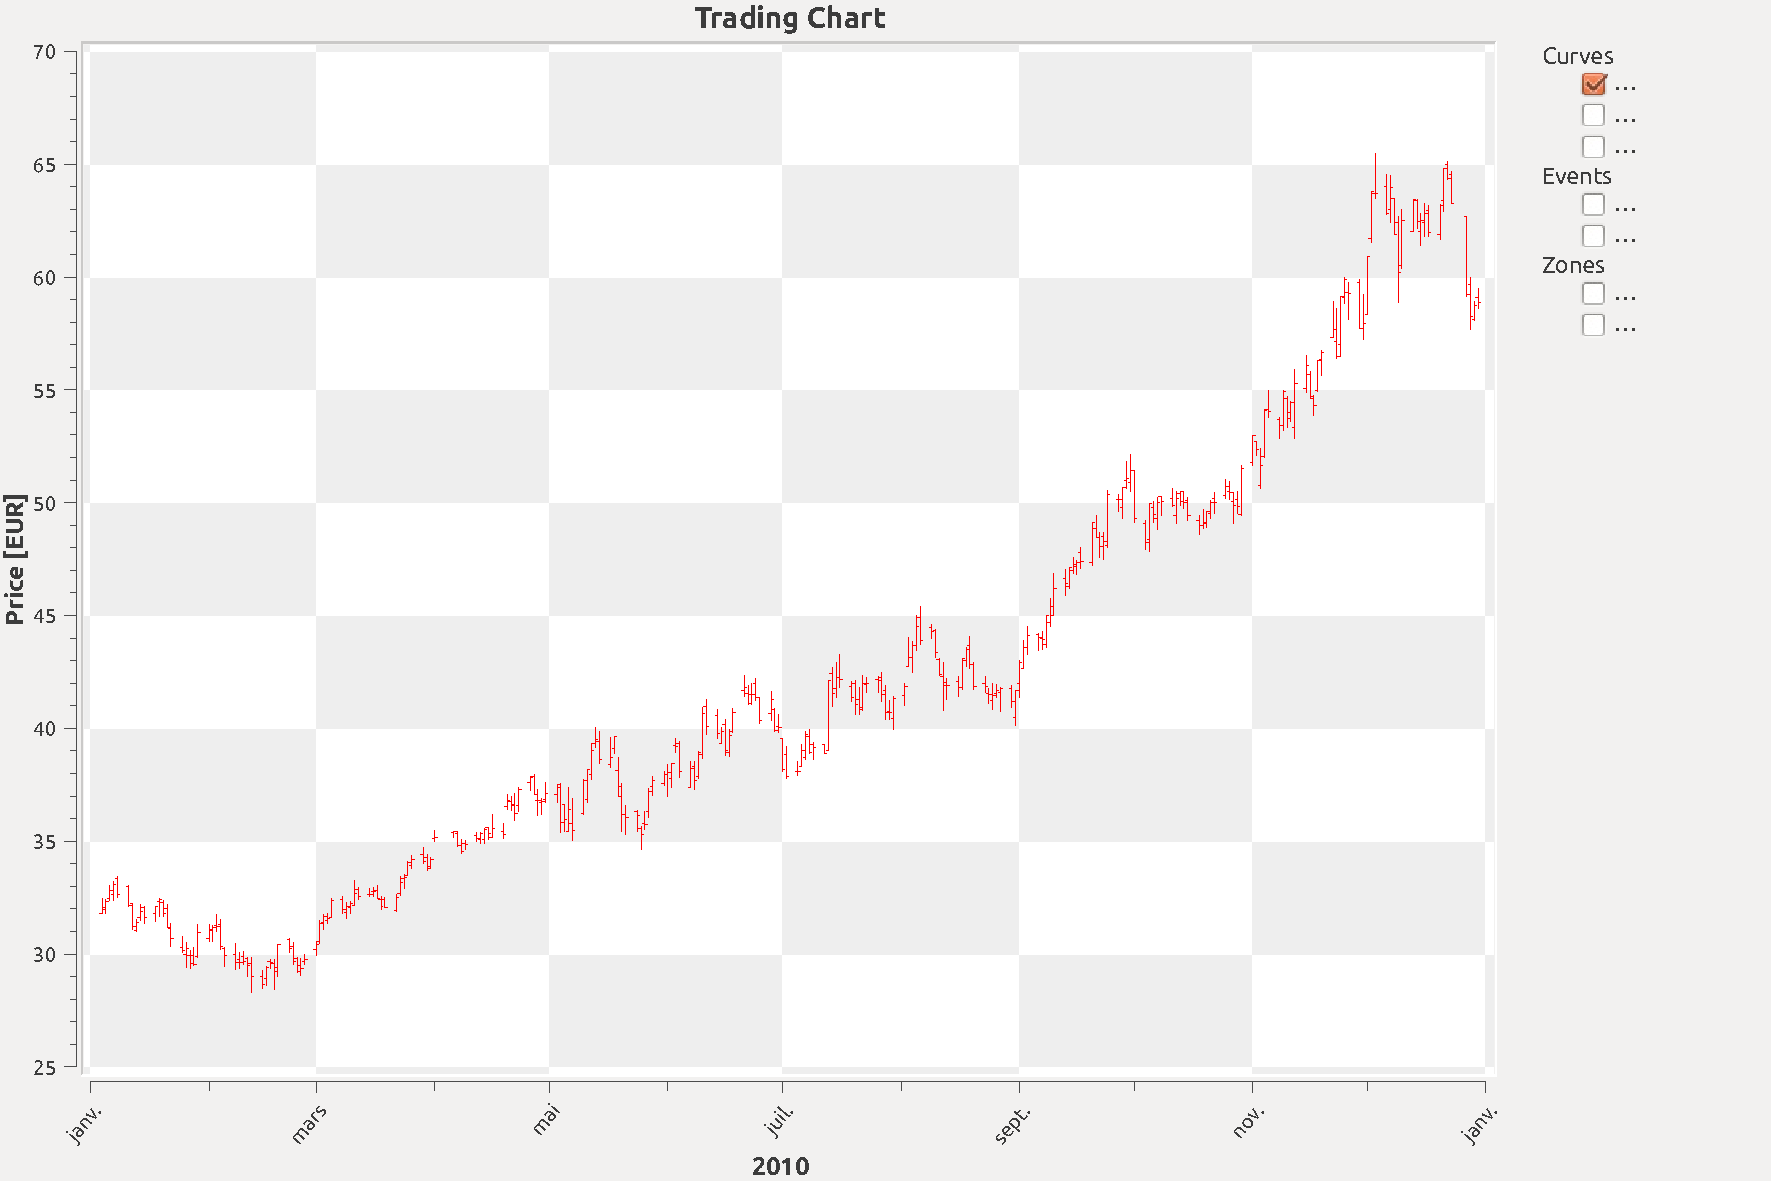
\includepdf[pages={1}]{stockchart.pdf}
%\section{Sample paper}\label{sec:Sample}
%\begin{figure}[htp] \centering{
%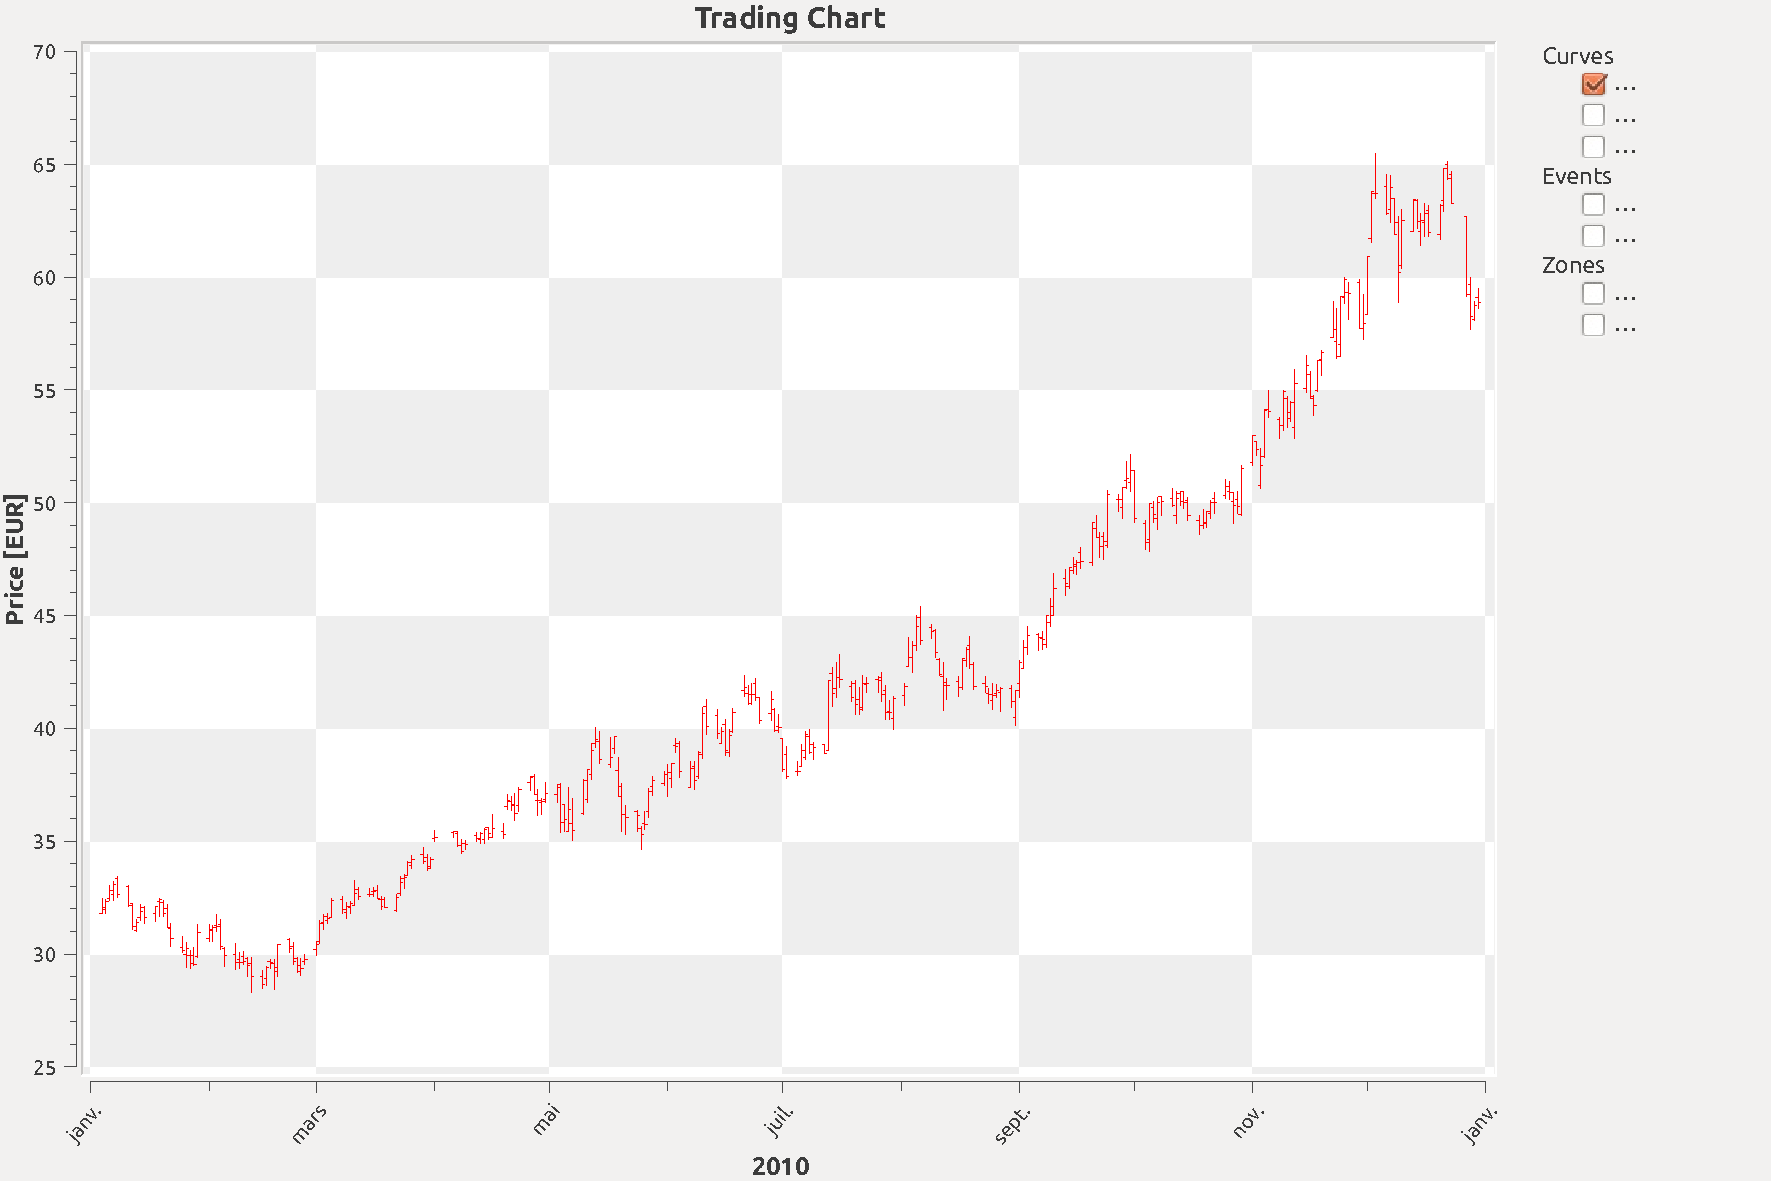
\includegraphics[scale=0.5]{stockchart.pdf}}
%\caption{Experiment 2}
%\end{figure}
\end{document}

\end{document}
